%auto-ignore
\renewcommand{\vec}[1]{\mathbf{#1}}

\usepackage{caption}
\usepackage{subcaption}
\usepackage{tabularx}
\usepackage{multirow}
\usepackage{amsmath}
\usepackage{tikz}
\usetikzlibrary{calc}
\usepackage{amssymb}
\usepackage{xcolor}
\usepackage{graphicx}
\usepackage{pgf}
\usepackage{pgfpages}
\usepackage{background}
\usepackage{algorithm}% http://ctan.org/pkg/algorithms
%\usepackage{algpseudocode}% http://ctan.org/pkg/algorithmicx
\usepackage{algpseudocode}



\usepackage{amsthm}           
\newtheorem{thm}{Theorem}[section]
\newtheorem{lem}[thm]{Lemma}
\newtheorem{prop}[thm]{Proposition}
\newtheorem{cor}[thm]{Corollary}
\newtheorem{conj}[thm]{Conjecture}
\newtheorem{mydef}[thm]{Definition}

\renewcommand{\vec}[1]{\mathbf{#1}}

\newcommand{\Pro}{\operatorname{Pr_0}}
\newcommand{\X}{\mathbf{X}}
\newcommand{\Y}{\mathbf{Y}}
\newcommand{\Z}{\mathbf{Z}}
\newcommand{\I}{\mathbf{I}}
\newcommand{\Ninst}{N\operatorname{inst}}
\newcommand{\inst}{\texttt{inst}}
\newcommand{\x}{\vec{x}}
\newcommand{\y}{\vec{y}}
\newcommand{\z}{\vec{z}}
\newcommand{\Lstuff}{\mathcal{L}_{\operatorname{stuff}}}
\newcommand{\Lthings}{\mathcal{L}_{\operatorname{things}}}


\newcommand{\Sim}{\operatorname{Sim}}


\newcommand{\zo}{\vec{z}_1}
\newcommand{\zt}{\vec{z}_2}
\newcommand{\Cm}{\mathbb{C}^m}

\newcommand{\mylist}[1]{\begin{enumerate}#1\end{enumerate}}
  
\newcommand{\bd}[1]{\textbf{#1}}
\newcommand{\imI}{\mathrm{i}}

\newcommand{\indemp}[1]{\index{#1}\emph{#1}}

\newcommand{\minuseq}{\mathrel{{-}{=}}}
\newcommand{\pluseq}{\mathrel{{+}{=}}}
\newcommand{\coleq}{\mathrel{{:}{=}}}
\newcommand{\cl}{\operatorname{class}}
\newcommand{\addborder}{
    \begin{tikzpicture}[remember picture, overlay]
        \draw[line width=1pt] 
            ($(current page.north west)+(0.5in,-0.5in)$) 
            rectangle 
            ($(current page.south east)+(-0.5in,1in)$);
    \end{tikzpicture}
}

%\newcommand*\Let[2]{\State #1 $\gets$ #2}
%\algrenewcommand\alglinenumber[1]{
%    {\sf\footnotesize\addfontfeatures{Colour=888888,Numbers=Monospaced}#1}}
%\algrenewcommand\algorithmicrequire{\textbf{Precondition:}}
%\algrenewcommand\algorithmicensure{\textbf{Postcondition:}}